\section{套筒三维模型构建}\label{sec:taotongjianmo}
基于上面的认识和理解,现在可以用AutoCAD来构建套筒的三维模型,具体构建方法是:
\begin{procedure}

\item 启动AutoCAD软件。

启动AutoCAD软件的方法通常有:
\begin{itemize}
\item 双击桌面图标
\includegraphics[scale=0.2]{cadicon.png}。
\item 【开始】$\rightarrow$ 【所有程序】$\rightarrow$【Autodesk】$\rightarrow$【AutoCAD 2013 – 简体中文 (Simplified Chinese)】$\rightarrow$【AutoCAD 2013 – 简体中文 (Simplified Chinese)】。
\end{itemize}
AutoCAD软件启动完成后,将出现图\ref{fig:cadui}所示的软件界面。
\begin{figure}[htbp]
\centering
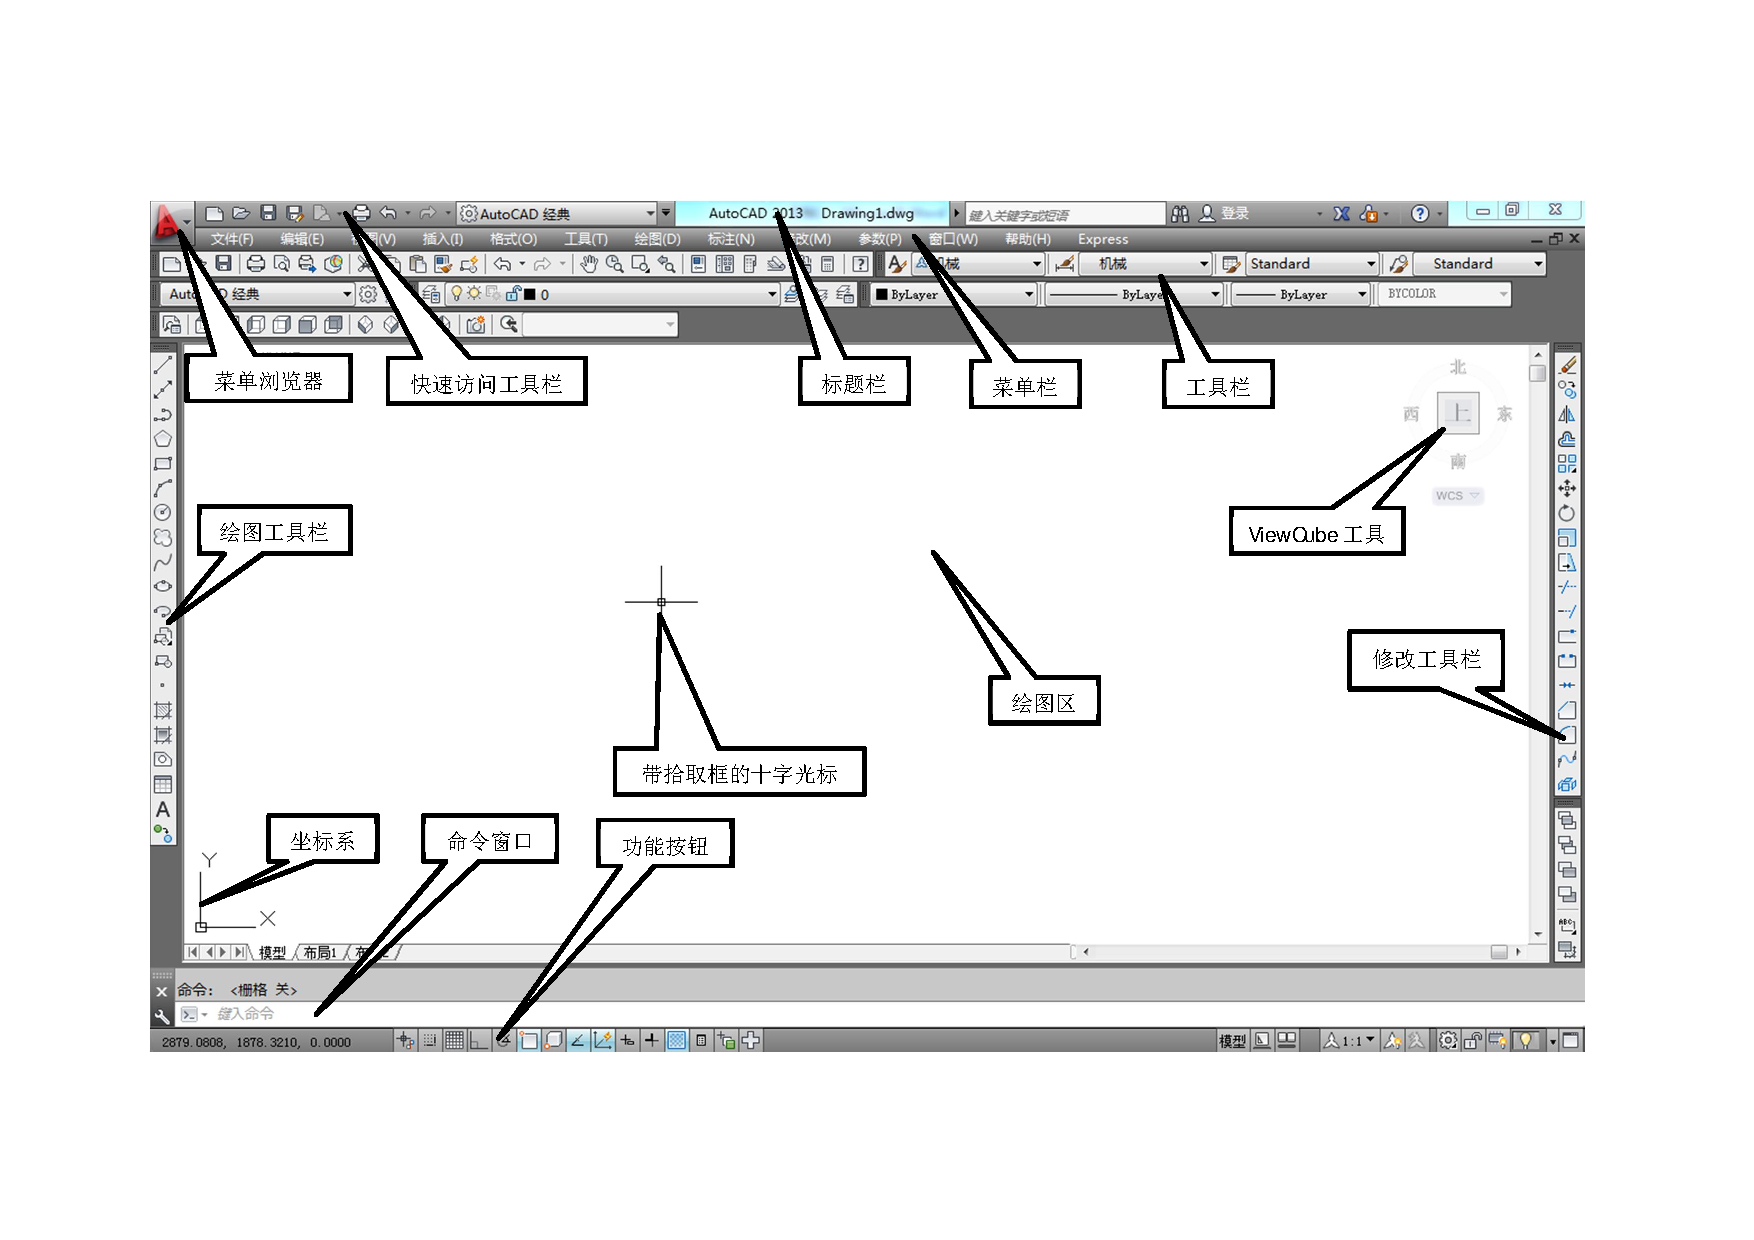
\includegraphics[scale=0.5]{cadui.pdf}
\caption{“AutoCAD经典”工作空间}\label{fig:cadui}
\end{figure}
AutoCAD软件的界面与Word字处理软件的界面非常相似,也是由标题栏、菜单栏、工具栏、绘图区、状态栏等要素构成。不同的是AutoCAD软件的界面在标题栏上还有菜单浏览器和快速访问工具栏;绘图区的左下方有坐标系,右上方有ViewCube工具,左边有绘图工具栏,右边有编辑工具栏;状态栏的上方有命令窗口;状态栏中有功能按钮。

\item 将视图切换为左视图。

AutoCAD启动后默认的视图方向是俯视图方向,而套筒零件的特征图位于左视图方向,为使套筒零件的三维模型与纸方向一致,需要将AutoCAD的视图方向切换为左视图方向。实现左视图切换的方法有:
\begin{itemize}
\item 键盘输入-VIME\index{-view,视图} 或-V,选择【正交】选项中的【左视】项。
\item 键盘输入-VIME,并输入left。
\item 【视图】$\rightarrow$【三维视图】$\rightarrow$【左视图】。
\item 【视图】$\triangleright$【左视】图标
\includegraphics[scale=0.6]{lefttool.png}。
\end{itemize}
同理,如果要将视图切换为其它视图方向,其操作方法与切换左视图的方法是一致的,只是需要将“左视”换成其它视图方向即可。例如要将视图方向切换为俯视图方向则将上述方法中的【左视】改为【俯视】。

\begin{lstlisting}
命令: -VIEW
输入选项 [?/删除(D)/正交(O)/恢复(R)/保存(S)/设置(E)/窗口(W)]: left
\end{lstlisting}

\yaodian{结合能够显著表达物体特征的视图选择AutoCAD的三维视图方向,将有助于三维模型的构建。}

\item 构建外圆柱
在AutoCAD中,创建圆柱体需要用到圆柱体命令,通常启动【圆柱体】命令的方法有:
\begin{itemize}
\item 键盘输入CYLINDER\index{cylinder,圆柱体}或CYL。
\item 【绘图】$\rightarrow$【建模】$\rightarrow$【圆柱体】。
\item 【建模】$\triangleright$【圆柱体】图标
\includegraphics[scale=0.6]{cylinder.png}。
\end{itemize}
在图\ref{fig:commandline}所示的命令行窗口中输入CYLINDER命令,并回车或按空格键结束命令。结束命令输入后,绘图区中的光标形状由带拾取框的十字光标“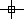
\includegraphics[scale=0.8]{guangbiao1} ”变成十字形光标“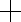
\includegraphics[scale=0.6]{guangbiao2}”,表示此时AutoCAD进入了绘图状态。
\begin{figure}[htbp]
\centering
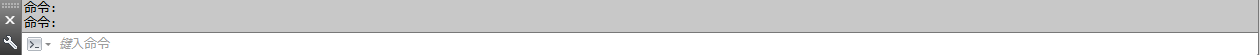
\includegraphics[scale=0.35]{commandline.png}
\caption{AutoCAD命令行}\label{fig:commandline}
\end{figure}

\yaodian{AutoCAD命令行是重要的信息窗口,是正确绘图的关键。初学者应多关注命令行的提示。}
\begin{lstlisting}
命令: _CYLINDER
\end{lstlisting}
接下来命令提示行中会提示,指定圆柱体的底面中心点或者绘图选项。
\begin{lstlisting}
指定底面的中心点或 [三点(3P)/两点(2P)/切点、切点、半径(T)/椭圆(E)]:
\end{lstlisting}
看到上述提示后,可以用鼠标在绘图区中任意单击一下,以完成底面中心点的指定,也可能输入其它选项来指定底面。

接下来,命令提示输入底面的半径,此时根据$\phi 14$直径尺寸计算得到半径应该是7,因此直接从键盘上输入数字7并按空格键或回车键结束半径的指定。如果要指定直径则需要在指定半径的提示下,输入选项字母D来进入指定直径状态。
\begin{lstlisting}
指定底面半径或 [直径(D)]: 7
\end{lstlisting}
最后,命令提示指定圆柱体的高度,此时从键盘上输入数字28,并按回车或空格键结束高度指定。
\begin{lstlisting}
指定高度或 [两点(2P)/轴端点(A)]: 28
\end{lstlisting}
此时,绘图区的光标切换为带拾取框的十字光标,表示AutoCAD当前处于非绘图命令状态。
\item 将视图方向切换为西南等轴测。
\begin{lstlisting}
命令: -VIEW
-VIEW输入选项 [?/删除(D)/正交(O)/恢复(R)/保存(S)/设置(E)/窗口(W)]:  swiso
\end{lstlisting}
完成视图切换后,可以看到图\ref{fig:taotong1} 所示的结果。
\begin{figure}[htbp]
\centering
\subfloat[]{\label{fig:taotong1}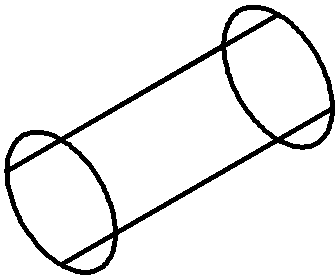
\includegraphics[scale=0.3]{taotong1.png}}\hspace{20pt}
\subfloat[]{\label{fig:centerselect}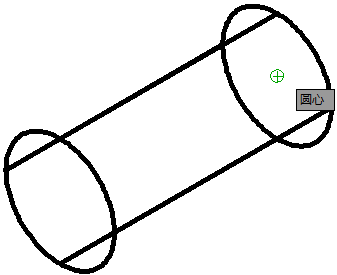
\includegraphics[scale=0.3]{centerselect.png}}\hspace{20pt}
\subfloat[]{\label{fig:taotong2}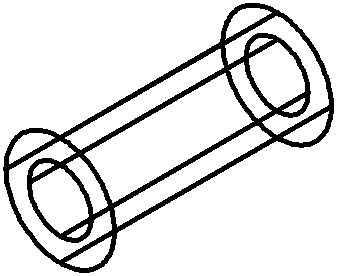
\includegraphics[scale=0.3]{taotong2.png}}
\caption{构建圆柱体}
\end{figure}

\item 构建内圆柱
\begin{lstlisting}
命令: _CYLINDER
指定底面的中心点或 [三点(3P)/两点(2P)/切点、切点、半径(T)/椭圆(E)]:
\end{lstlisting}
当命令提示指定底面圆心时,为保证我们所绘制的$\phi 8$圆柱与$\phi 14$圆上下端面对齐并且同轴,需要应用AutoCAD的对象后捕捉方式来选取$\phi 14$圆底端面的圆心作为$\phi 8$圆柱底端面的圆心。其具体操作方法是:将鼠标移至图\ref{fig:centerselect}所示的位置,直到出现图示的圆心标记和提示,然后单击鼠标左键确定圆柱体的圆心,并按下面的提示完$\phi 8$圆柱体的构建。
\begin{lstlisting}
指定底面半径或 [直径(D)] <7.0000>: 4
指定高度或 [两点(2P)/轴端点(A)] <28.0000>:
\end{lstlisting}

\yaodian{合理使用捕捉是实现精确绘图和快速绘图的重要方法之一。}

\item 进行差集操作,制作内孔

由于前面构建的是两个实体的圆柱体,因此并没有真构成套筒零件所需要的孔,而实现孔的构建则需要从$\phi 14$的圆柱体中去除一个$\phi 8$的圆柱体,要实现这一目标,需要用到实体编辑中的【差集】命令,其启动方法有:
\begin{itemize}
\item 键盘输入SUBTRACT\index{subtract,差集}或SU。
\item 【修改】$\rightarrow$【实体编辑】$\rightarrow$【差集】。
\item 【实体编辑】$\triangleright$【差集】图标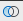
\includegraphics[scale=0.7]{subtracttool.png}。
\end{itemize}
\begin{figure}[htbp]
\centering
\subfloat[]{\label{fig:subtractselect}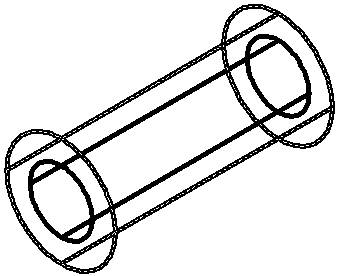
\includegraphics[scale=0.3]{subtractselect.png}}\hspace{40pt}
\subfloat[]{\label{fig:subtractselect1}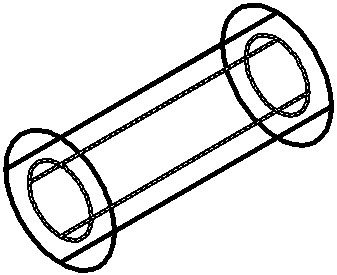
\includegraphics[scale=0.3]{subtractselect1.png}}
\caption{差集操作}
\end{figure}
\begin{lstlisting}
命令: SUBTRACT
选择要从中减去的实体、曲面和面域...
\end{lstlisting}
输入SUBTACT命令后,提示选择要从中减去的实体,同时绘图区的鼠标形状变为矩形小方框“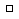
\includegraphics[scale=0.8]{selectobject.png}”,表示进入选择对象状态,此时按照图\ref{fig:subtractselect}所示选择$\phi 14$的圆柱体作为要从中减去的对象,并按回车或空格键结束选择。
\begin{lstlisting}
选择对象: 找到 1 个
选择对象:  选择要减去的实体、曲面和面域...
\end{lstlisting}
结束从中减去实体选择后,命令提示选择要减去的实体,此时按照图\ref{fig:subtractselect1}所示选择$\phi 8$圆柱体作为要选择的实体,并按驾车可空格键结束选择。
\begin{lstlisting}
选择对象: 找到 1 个
选择对象:
\end{lstlisting}
\item 进行倒角操作
至此,已经完成了套筒的整体部分的构建,还剩下两个倒角没有完成,在AutoCAD中完成三维立体倒角边构建的命令是“倒角边”,其启动方法有:
\begin{itemize}
\item 键盘输入CHAMFEREDGE\index{charmferedge,倒角边}。
\item 【修改】$\rightarrow$【实体编辑】$\rightarrow$【倒角边】。
\item 【实体编辑】$\triangleright$【倒角边】图标
\includegraphics[scale=0.6]{chamferedge.png}。
\end{itemize}

\begin{lstlisting}
命令: CHAMFEREDGE
距离 1 = 1.0000,距离 2 = 1.0000
\end{lstlisting}
启动完倒角边命令后,命令会提示当前的倒角边距离的默认值,并提示选择要倒角的边,此时按照图\ref{fig:chamferedgeselect}所示选择要倒角的一条边,选择完成后会自动生成倒角预览。
\begin{figure}[htbp]
\centering
\subfloat[]{\label{fig:chamferedgeselect}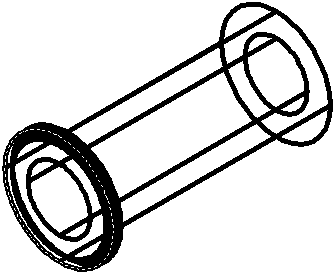
\includegraphics[scale=0.3]{chamferedgeselect.png}}\hspace{20pt}
\subfloat[]{\label{fig:chamferedgeselect1}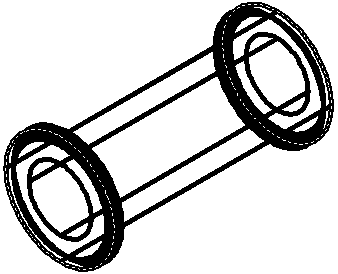
\includegraphics[scale=0.3]{chamferedgeselect1.png}}
\hspace{20pt}
\subfloat[]{\label{fig:chamferedgeresult}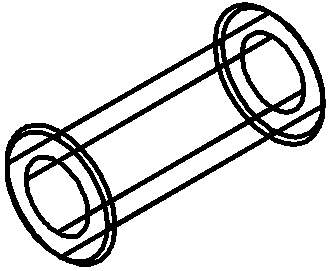
\includegraphics[scale=0.3]{chamferedgeresult.png}}
\caption{倒角边操作}
\end{figure}
\begin{lstlisting}
选择一条边或 [环(L)/距离(D)]:
\end{lstlisting}
接下来,按照图\ref{fig:chamferedgeselect1}所示,选择另一条要倒角的边。
\begin{lstlisting}
选择同一个面上的其他边或 [环(L)/距离(D)]:
\end{lstlisting}
套筒零件只有两个倒角边,因此选择倒角边至此结束,但是系统默认值并不是需要的倒距离,故需要选择距离(d)进行修改。
\begin{lstlisting}
选择同一个面上的其他边或 [环(L)/距离(D)]:d
\end{lstlisting}
最后将两个倒角距离均设置成为0.5,并用回车键接受,其结果如图\ref{fig:chamferedgeresult}所示。
\begin{lstlisting}
指定基面倒角距离或 [表达式(E)] <1.0000>: 0.5
指定其他曲面倒角距离或 [表达式(E)] <1.0000>: 0.5
按 Enter 键接受倒角或 [距离(D)]:
\end{lstlisting}
\item 进行着色
\begin{figure}[htbp]
\centering
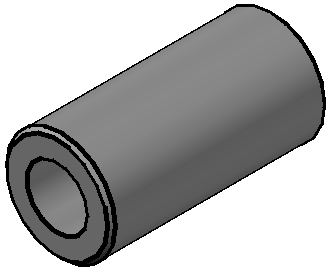
\includegraphics[scale=0.6]{taotonglititu.png}
\caption{套筒三维模型}\label{fig:taotonglititu}
\end{figure}
最后,将完成套筒三维模型以灰度方式的视觉样式进行着色,以使得三维模型看起更加真实。启动灰度视觉样式的方法有:
\begin{itemize}
\item 键盘输入 VSCURRENT\index{vscurrent,视觉样式}或VS,并输入G选项。
\item 【视图】$\rightarrow$【视觉样式】$\rightarrow$【灰度】。
\end{itemize}
\begin{lstlisting}
命令: vscurrent
输入选项 [二维线框(2)/线框(W)/隐藏(H)/真实(R)/概念(C)/着色(S)/带边缘着色(E)/灰度(G)/勾画(SK)/X 射线(X)/其他(O)] <二维线框>: G
\end{lstlisting}
完成灰度视觉样式切换后,其结果如图\ref{fig:taotonglititu}所示。

\end{procedure}

\endinput